\documentclass{article}
\usepackage[UTF8]{ctex}
\usepackage{amsmath}
\usepackage{amssymb}
\usepackage{graphicx}
\usepackage{geometry}
\geometry{a4paper, margin=2cm}

\newcommand{\problemname}[1]{\begin{center}\Large\bfseries #1\end{center}}
\usepackage{enumitem}

\begin{document}
\problemname{程序改错}

\textbf{注意}：这是一道标准的程序设计题目，代码已经给出，通过这道题目，我们来感受一下 \textbf{测评机的判分模式} 以及 \textbf{解决程序设计类问题的步骤} 。仔细读题后，思考：这个程序正确吗？

输入三个整数，并输出他们的乘积。

\subsection*{输入格式}
输入为一行，包括了用空格分隔的三个整数 $a$、$b$、$c$（ $1\lea,b,c,\le10000$ ）。

\subsection*{输出格式}
输出为一行，其中包含一个整数，是 $a$、$b$、$c$ 三个整数的乘积。

\begin{center}
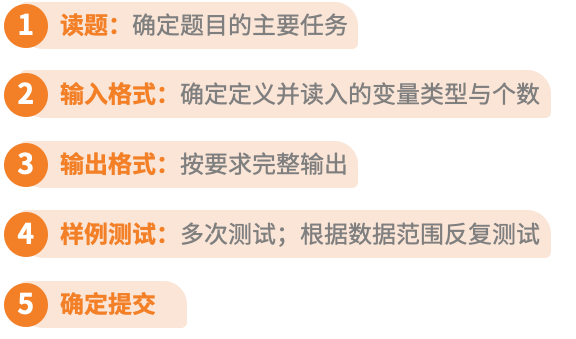
\includegraphics[width=0.7\textwidth]{suanfa35927-77653c769447fd35e41f.png}
\end{center}

\subsection*{样例输入}
\begin{verbatim}
1 2 3
\end{verbatim}

\subsection*{样例输出}
\begin{verbatim}
6
\end{verbatim}


\end{document}
